\documentclass[12pt]{article}
\usepackage{geometry}
\geometry{letterpaper, left=22.5mm, right=22.5mm, top=30mm, bottom=30mm}
\geometry{letterpaper}
\usepackage{amsmath}
\usepackage{amssymb}
\usepackage{enumitem}
\usepackage{fancyhdr}
\usepackage{framed}
\usepackage{tikz}
\usepackage{mathpazo}
%\usepackage{charter}
%\usepackage{newcent}
\usepackage{indentfirst}
\usepackage{booktabs}
\usepackage{graphicx}
\usepackage{float}
\usepackage{makecell}
\usepackage{xcolor}
\usepackage{mdframed}
\usetikzlibrary{trees}
\pagestyle{fancy}
\usepackage{amsthm}
\theoremstyle{definition}
\newtheorem{definition}{Definition}[section]
\theoremstyle{property}
\newtheorem{property}{Property}[section]
\theoremstyle{assumption}
\newtheorem{assumption}{Assumption}[section]
\theoremstyle{example}
\newtheorem{example}{Example}[section]
\theoremstyle{comment}
\newtheorem{comment}{Comment}[section]
\newtheorem{theorem}{Theorem}[section]
\newtheorem{corollary}{Corollary}[theorem]
\newtheorem{lemma}[theorem]{Lemma}
\usepackage{lastpage}
\usepackage{wrapfig}
\usepackage{hyperref}
\usepackage{subcaption}
\usepackage{setspace}
\hypersetup{
colorlinks=true,
linkcolor=black,
filecolor=green, 
urlcolor=blue,
}
\newcommand{\ROM}[1]
    {\MakeUppercase{\romannumeral #1}}
\fancyhead[L]{Econometrics \ROM{2}: Recitation 11 }%change each reci
\fancyhead[R]{Spring 2020}
\fancyfoot[C]{\thepage \hspace{1pt} / \pageref{LastPage}}

\fancypagestyle{firstpage}{%
\fancyhf{}%
\renewcommand{\headrulewidth}{0mm}%
  \fancyfoot[C]{\thepage \hspace{1pt} / \pageref{LastPage}}
}
%change title each rec
\title{Introduction to Econometrics \ROM{2}: Recitation 11\footnote{This is based on the lecture notes of Professors Jushan Bai and Bernard Salanie. I was also greatly helped by previous recitation notes from Paul Sungwook Koh and Dong Woo Hahm. The remaining errors are mine. }}

\begin{document}
\linespread{1.25}
\onehalfspacing

\author{Seung-hun Lee\footnote{Contact me at \href{mailto:sl4436@columbia.edu}{sl4436@columbia.edu} if you spot any errors or have suggestions on improving this note.}}
\date{April 22nd, 2020}
\maketitle
\thispagestyle{firstpage}

%%%%%%%%%%%%%%%%%%
\section{Discussion on the Conditional Independence Assumption}
\subsection{Violation of Conditional Independence Assumptions}
There are cases where the assignment, even if we condition on observables, are not random. So in the regressional framework of $y_{i}(d)=\mu(X_i,d)+\epsilon_i(d)$, the error terms is not independent of $D_i|X_i$. The conditional independence assumption can be broken because:
\begin{itemize}
\item Participants self-select based on expected benefit: Think about a job training program for plumbing. Then, maybe those who are more healthy and suffer less in terms of costs are likely to join. If health is not perfectly observed, we risk breaking the conditional independence assumption
\item Participants may be selected, consciously or not, to join: Think of the clinical trial where participation is voluntary. In such case, individuals who are more risk-loving are more likely to join. In other words, participants and nonparticipants systematically differ on risk-averseness - something that is not usually observed.
\item There may be equilibrium effects: A tuition subsidy program that intends to increase the number of people entering college may have a spillover effect by increasing supply of college graduates at the labor market, leading to a decrease in college premium. This may induce students to enter college less. If TE is the (rate of) college entrance, such equilibrium effect may be influential.  
\end{itemize}
\par
Mathematically, what happens is that when we calculate $E[Y_i|D_i=1,x]-E[Y_i|D_i=0,x]$, we end up with
\begin{align*}
E[Y_i|D_i=1,x]-E[Y_i|D_i=0.x]&=\mu(x.1)-\mu(x,0)+E[\epsilon_i(1)|D_i=1,x]-E[\epsilon_i(0)|D_i=0,x]\\
&=TE+E[\epsilon_i(1)|D_i=1,x]-E[\epsilon_i(0)|D_i=0,x]
\end{align*}
The error term no longer can be erased from the equation since CIA assumption is not applicable. The difference between the error term is the \textbf{selection bias} (Also appears in Angrist, Pischke 2009). This also means that the error terms and the $u_i$ in $D_i=1(u_i<p(x_i))$ can covary. The result is that the treatment effect estimated from here can be inaccurate. \par
There are two possible solutions. Old method relies on \textbf{Heckman correction}. Recent focus is on IV to derive \textbf{marginal treatment effects} and \textbf{localized average treatment effect}.
\subsection{A Brief Discussion of the Heckman Correction}
Suppose that we are in the situation where we have a data generating process
\[
Y_i = \max\{X_i\beta+\sigma\eta_i, 0\}, \eta_i \sim N(0,1)
\]
So we only see $Y_i$ if $X_i\beta+\sigma\eta_i>0$. We are able to observe $D_i$, specified as
\[
D_i=\begin{cases}1 & \text{if }\eta>-\frac{X_i\beta}{\sigma}\\ 0 & \text{otherwise} \end{cases}
\]
Then, for the observed sample, we are likely to have an $\eta_i$ that is positively selected. So the idiosyncratic error is no longer random and we have a biased estimates, shown as (assuming $X_i$ is observable)
\footnotesize{\begin{align*}
E[Y_i|Y_i>0]&= X_i\beta + E[\sigma\eta_i|Y_i>0]\\
\implies E[\eta_i|Y_i>0]& =E\left[\eta_i| \eta_i>-\frac{X_i\beta}{\sigma}\right]=\int_{-X_i\beta/\sigma}^\infty t\phi(t|\eta_i>-X_i\beta/\sigma)dt\\
&=\int_{-X_i\beta/\sigma}^\infty t\frac{\phi(t)}{\Pr(\eta_i>-X_i\beta/\sigma)}dt =\frac{1}{1-\Phi(-X_i\beta/\sigma)}\int_{-X_i\beta/\sigma}^\infty t\frac{1}{\sqrt{2\pi}}e^{-t^2/2}dt\\
&=\frac{1}{1-\Phi(-X_i\beta/\sigma)}\left[\frac{1}{\sqrt{2\pi}}e^{-t^2/2}\right]_{-X_i\beta/\sigma}^\infty=\frac{\phi(-X_i\beta/\sigma)}{1-\Phi(-X_i\beta/\sigma)}\\
&=\frac{\phi(X_i\beta/\sigma)}{\Phi(X_i\beta/\sigma)}=m(-X_i\beta/\sigma)\neq0\\
\end{align*}}\normalsize
So the error has nonzero conditional mean. The ratio of the pdf over cdf $\frac{\phi(\cdot)}{\Phi(\cdot)}$ is the inverse Mill's ratio (IMR). Heckman's correction uses the IMR to correct for the bias. The challenge is to identify $\beta/\sigma$. We do this by
\begin{enumerate}
\item Use probit to regress $D_i$ onto $X_i$. Then we can obtain $\widehat{\beta/\sigma}$.
\item Define $\hat{f}(x)=m(-X_i\widehat{\beta/\sigma})$. We include $\hat{f}(x)$ in the control variable and run
\[
Y_i = X_i\beta+ \gamma\hat{f}(x)+\epsilon_i
\]
on the participant sample. 
\end{enumerate}\par
The problem is that we assume the normality of the error term and the linearity of the DGP, which is not always true. Thus, it is not always an ideal way to deal with selection on unobservables. 
\subsection{Instrumental Variables}
In this setup, you assume that there exist variables $Z_i$ that affect the treatment $D_i$ but not the outcomes (at least on its own). It should satisfy
\begin{itemize}
\item \textbf{Relevancy}: It effects the propensity score $p(x,z)=\Pr(D_i=1|X_i=x, Z_i=z)$
\item \textbf{Validity}: Distribution of the counterfactual outcomes and $u_i$ does not depend on $Z_i|X_i$. To put it in mathematical notation, 
\[
(Y_i(1), Y_i(0), u_i) \perp \!\!\!\perp Z_i|X_i
\]
\begin{mdframed}[backgroundcolor=yellow!5] 
\begin{comment}[Some remarks about the above condition] Note that $u_i$ is tied together with the potential outcomes. This implies that $u_i$ and the outcome can be correlated, which is allowed in a non-CIA setup. What matters is that the changes in $Z_i$ not affect $u_i$
\end{comment}
\begin{comment}[Violation of validity]  Let $Z_i$ change from $z$ to $z'>z$ and that the propensity rises with $z$. Suppose that for a fixed $X_i=x$, $p(x,z)>u_i$. So $D_i=1$ in this case. If we have $p(x,z')<u_i'$, then $D_i=0$. In addition, we may have the change of $z$ itself affecting the outcome directly with the violation of the validity condition.  
\end{comment}
\begin{comment}[So who are we identifying?] If $u$ is independent of $Z_i$ given $X_i$, then by moving from $p(x,z)$ to some $p(x,z')$, we can find a group of individuals who do not get treated at $p(x,z)$ but do get treated at $p(x,z')$. We refer to them as \textbf{compliers}. If people were participating at $p(x,z)$ they participate at $p(x,z')$. We then have a group of \textbf{always takers}. Conversely, if people do not get treated at $p(x,z')$, they don't get treated at lower propensity scores - the \textbf{never takers}. \par
We do not identify \textbf{defiers} - they have $u_i<p(x,z)$ but $u_i'>p(x,z')>p(x,z)$. The only way this can happen is if $u_i$ changes with $z_i$ - a violation of validity. This is sometimes called as monotonicity condition or no two-way movement condition. 

\end{comment}
\end{mdframed}
\item \textbf{Full support}: The support of $p(x,z)$ conditional on $x$ extends to all of $[0,1]$. This implies that change in $Z$ induces large variations in the propensity score. 
\end{itemize} 
\par
So what concerns do we run into in terms of identification? We can identify $p(x,z)$ by calculating $\Pr(D_i=1|X_i=x, Z_i=z)$. We can also write
\begin{align*}
E[Y_i|D_i=1, X_i=x, Z_i=z]&=\mu(x,1)+E[\epsilon_i(1)|u_i<p(x,z), X_i=x, Z_i=z]\\
&=\mu(x,1)+E[\epsilon_i(1)|u_i<p(x,z), X_i=x] \ (\because\text{validity})
\end{align*}
Define $K_1(p(x,z))=E[\epsilon_i(1)|u_i<p(x,z), X_i=x]$ to be some unknown function of the conditional expectation of $\epsilon_i(1)$. We can also work similarly to define 
\[
E[Y_i|D_i=0, X_i=x, Z_i=z]=\mu(x,0)+E[\epsilon_i(0)|u_i>p(x,z), X_i=x]
\] 
and $K_0(p(x,z))=E[\epsilon_i(0)|u_i>p(x,z), X_i=x]$. Note that the left hand sides for both sets of equations can be identified by naively taking an average of $Y_i$'s conditional on some the treated (untreated) for the group $X_i=x, Z_i=z$. The estimated result breaks down into
\[
\mu(x,1)-\mu(x,0)+\underbrace{K_1(p(x,z))-K_0(p(x,z)) }_{\Delta(p(x,z))}= TE(x)+\Delta(p(x,z))
\]
The $\Delta(p(x,z))$ is the control function that stands for the selection bias. By the relevance condition, the change in $z$ affects the value of $p(x,z)$ for a fixed $x$. So changing $z$ allows us to identify how $\Delta(p(x,z))$ \textit{changes}. However, we do not know what the \textit{exact value} of $\Delta(p(x,z))$ is for the initial value of $z$ we started. Therefore, the true parameter of interest, which is TE, cannot be uncovered. \par
So how can we progress on? Note that the $K_d$ functions are conditional expectations of $\epsilon_i(d)$ on $X_i=x$ and selection rule $u_i (<,>) p(x,z)$. In particular, we can get that
\begin{align*}
K_1(1) &=E[\epsilon_i(1)|u_i<1,X_i=x] \\
&=E[\epsilon_i(1)|X_i=x] \ (\because\text{Everyone is treated})\\
&=0\\
K_0(0) &=E[\epsilon_i(1)|u_i>0,X_i=x] \\
&=E[\epsilon_i(1)|X_i=x] \ (\because\text{No one is treated})\\
&=0
\end{align*}
Heckman and Vytlacil show that if we are given a continuous instrument $z$, we can do a much better job of identifying the treatment effect. 
\subsection{Marginal Treatment Effects}
The \textbf{marginal treatment effect} at $p(x,z)=p$ is defined as the treatment effect on individuals whose $u_i=p(x,z)$. We can write
\[
MTE(p)=E[Y_i(1)-Y_i(0)| u_i=p]
\]
The conditional expectation above is not directly obtainable from the data. Heckman and Vytlacil show that 
\[
MTE(p)=\frac{\partial E[Y_i | p(x,z)=p]}{\partial p}
\]
which is obtainable from the data. This is done by 
\begin{enumerate}
\item Estimate $p(x,z)=\Pr(D_i=1|X_i=x. Z_i=z)$
\item Regress $Y_i$ on the estimated $p(x,z)$ in a flexible setting - preferably not just linearly but with some nonlinearities
\item Take a derivative with respect to $p$. (or local linear estimator)
\item For treatment effects, evaluate the $E[Y_i|p(x,z),x]$ at $p(x,z)=1$ and $p(x,z)=0$ and identify the difference. (You can obtain $E[Y_i|\cdot]$ by getting the predicted values).  
\end{enumerate}
\par
Intuitively, what is going on with MTE is as follows: By changing $p$ slightly by $dp$, we are able to identify the marginal compliers who move from not being treated to being treated. We are finding out how their outcome changes as they move from non-participation to participation into the treatment. \par
To see why the above result holds, we define
\[
G(p)=E[Y_i\cdot 1(p(x,z)=p)]
\]
Since $Y_i=D_iY_i(1)+(1-D_i)Y_i(0)=1(u_i<p(x,z))Y_i(1)+1(u_i>p(x,z))Y_i(0)$, we can rewrite the above as
\begin{align*}
G(p)&=E[Y_i(1)\cdot 1(u_i<p(x,z))\cdot 1(p(x,z)=p)+Y_i(0)\cdot 1(u_i>p(x,z))\cdot 1(p(x,z)=p)]\\
&=E[Y_i(1)\cdot 1(u_i<p)\cdot 1(p(x,z)=p)]+E[Y_i(0)\cdot 1(u_i>p)\cdot 1(p(x,z)=p)]\\
&=G_1(p)+G_0(p)
\end{align*}
By the validity condition and the fact that $u_i\sim U[0,1]$ (and thus $f(u_i)=1$), we can write
\begin{align*}
E[Y_i(1)\cdot 1(u_i<p)\cdot 1(p(x,z)=p)]&=E[Y_i(1)\cdot 1(u_i<p)]\Pr(p(x,z)=p)\\
&=\int_0^pE[Y_i(1)|u=t]dt\Pr(p(x,z)=p)
\end{align*}
And similarly, 
\[
E[Y_i(0)\cdot 1(u_i>p)\cdot 1(p(x,z)=p)]=\int_p^1E[Y_i(0)|u=t]dt\Pr(p(x,z)=p)
\]
So 
\footnotesize{\[
E[Y_i\cdot 1(p(x,z)=p)]=G(p)=\left(\int_0^pE[Y_i(1)|u=t]dt+\int_p^1E[Y_i(0)|u=t]dt\right)\Pr(p(x,z)=p)
\]}\normalsize
with the fact that $E[Y_i\cdot 1(p(x,z)=p)]=E[Y_i|p(x,z)=p]\cdot \Pr(p(x,z)=p) $ this implies that
\footnotesize{\[
E[Y_i|p(x,z)=p]=\frac{G(p)}{\Pr(p(x,z)=p)}=\int_0^pE[Y_i(1)|u=t]dt+\int_p^1E[Y_i(0)|u=t]dt
\]}\normalsize
Then, by Leibniz's integral rule
\[
\frac{\partial E[Y_i | p(x,z)=p]}{\partial p}=E[Y_i(1)|u=p]-E[Y_i(0)|u=p]=MTE(p)
\]
Hence, the treatment effect can be recovered by
\[
TE=\int_0^1MTE(p)dp=E[Y_i|p(x,z)=1]-E[Y_i|p(x,z)=0]
\]

\subsection{Some Large Caveats}
For the above methods to work, we need the $Z_i$ instruments to satisfy
\begin{itemize}
\item $Z$ belongs in the treatment equation (relevancy): $D_i=1(u_i<p(X_i,Z_i))$
\item $Z$ does not belong in the outcome equation (exclusivity): $Y_i(d)=\mu(x,d)+\epsilon_i(d)$
\item In other words, we get $(\epsilon_i(1), \epsilon_i(0), u_i) \perp\!\!\!\perp Z_i|X_i$
\item Continuity: $p(x,z)$ changes w.r.t $z$ in a continuous way (This is because we need to be able to take derivatives)
\end{itemize}
For the range of $p(x,z)$ available, the above condition allows us to estimate the marginal treatment effect. For any work you see that uses marginal treatment effect, there includes a graph that maps marginal treatment effect on the vertical axis and the `resistance' parameter $u_i$ on the horizontal axis. \par
With this framework, we can also test if conditional independence assumption holds. Recall that conditional independence assumption is satisfied when
\[
(\epsilon_i(1),\epsilon_i(0)) \perp\!\!\!\perp u_i|X_i
\]
In cases where this is true, then the outcomes are independent of $u_i$ conditional on $X_i$. Thus, 
\[
MTE(x,p)=E[Y_i(1)-Y_i(0)|X_i=x, u_i=p]=E[Y_i(1)-Y_i(0)|X_i=x]
\]
Since $MTE(x,p)=\frac{\partial E[Y_i | X_i=x, p(x, z)=p]}{\partial p}$, the above condition implies that $E[Y_i|X_i=x, p(x, z)=p]$ is linear in $p$. Thus, it is highly recommended to put polynomial terms of $p^k, k=1,2,3,...$ when you estimate marginal treatment effects. Then, test to find whether the nonlinear terms have coefficient zero. 
\par 
So what do we gain by testing the form of $MTE(x,p)$? How it varies with $p$ may inform how well the treatment is designed. Ideally, we want the treatment to be applied to those who are more likely to be benefitted by it. If $p$ is higher for those with larger benefits, then the design is well-targeted.
\begin{mdframed}[backgroundcolor=blue!5] 
\begin{definition}[Policy Relevant Treatment Effect]  Policy relevant treatment effect is the mean effect of going from a baseline policy to a new policy per net person shifted (Heckman, Vytlacil 2001, Carneiro, Heckman, Vytlacil 2010). This can be written as
\begin{gather*}
\frac{E[Y_i|\text{New Policy}]-E[Y_i|\text{Old Policy}]}{E[D_i|\text{New Policy}]-E[D_i|\text{Old Policy}]}\\
=\int_0^1MTE(u)\omega(x,u) du\  \  \ \ (\omega(x,u)=F_{P_{old}|X}(u|x)-F_{P_{new}|X}(u|x))
\end{gather*}
\end{definition}
\end{mdframed}

\begin{mdframed}[backgroundcolor=yellow!5] 
\begin{example}[Carneiro \& Lee, 2019] The paper estimates the impact of attending college on log wage distributions. The paper finds that individuals more likely to attend college (and have low resistance parameters) are more likely to have higher college wage ($Y_i(1)$) over high school wage ($Y_i(0)$). The opposite holds true for people with high school degree. They have a MTE figure (at figure 3) that maps MTE as a function of resistance parameters.
\end{example}
\begin{example}[Johnson \& Taylor, 2019] The paper shows that causal impact of migration decreases longevity. This is even with the consideration that migrants are more likely to be educated and have higher baseline earnings compared to non-migrants. They use the MTE to (with railcar traffic at the town of origin as one of their IVs). They document that those who have lower latent ability (high $U_d$) suffer more from migrating out, reflected in the downward sloping MTE 
\end{example}
\centering
\begin{figure}[H]
\begin{subfigure}{0.5\textwidth}
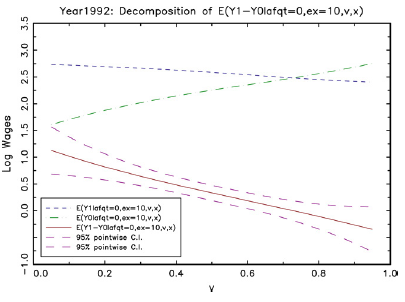
\includegraphics[width=\textwidth]{fig11_1}
\caption{Carneiro, Lee (2009)}
\end{subfigure}
\begin{subfigure}{0.5\textwidth}
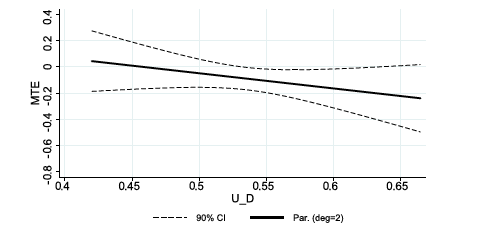
\includegraphics[width=\textwidth]{fig11_2}
\caption{Johnson, Taylor (2019)}
\end{subfigure}
\end{figure}
\end{mdframed}
\subsection{Local Average Treatment Effect}
The marginal treatment effect looks at `marginal' compliers: It is interested in the small group of individuals who changes treatment status from $D_i=0$  to $D_i=1$ as $p(x,z)$ changes slightly due to $Z_i$. Instead of changing the propensity score by a tiny bit (thanks to the continuity of the instrument $Z_i$), we can look at finite differences - like $Z_i$ having just two possible values. Then we are going to be looking at a larger group of compliers than in the marginal treatment effect context. The treatment effect for this larger group of compliers is called \textbf{local average treatment effect}. \par
We will setup the framework as follows:
\begin{itemize}
\item $Z_i$ will be a binary instrumental variable. This of this as an eligibility rule. 
\item $D_i(z)$ can be characterized as $D_i(z)=1(u_i<p(x,z))$. Note that as $z$ rises, so will $p(x,z)$. This is the relevance condition
\item $Z_i$ itself has no bearing, at least directly, on the outcome. So $Y_i(d)=\mu(x,d)+\epsilon_i(d)$. So we still have $(\epsilon_i(1), \epsilon_i(0), u_i)\perp\!\!\!\perp Z_i|X_i$. 
\end{itemize}
The formal way to define local average treatment effect is as follows
\[
LATE(x)=E[Y_i(1)-Y_i(0)|p(x,z)<u_i<p(x,z'). X_i=x]
\]
We can identify LATE by using the following (I skip $X_i=x$)
\footnotesize{\begin{align*}
E[Y_i|Z_i=z']-E[Y_i|Z_i=z]&=E[1(u_i<p(z'))Y_i(1)+1(u_i>p(z'))Y_i(0)|Z_i=z']\\
&-E[1(u_i<p(z))Y_i(1)+1(u_i>p(z))Y_i(0)|Z_i=z]\\
&=E[1(u_i<p(z'))Y_i(1)+1(u_i>p(z'))Y_i(0)]\\
&-E[1(u_i<p(z))Y_i(1)+1(u_i>p(z))Y_i(0)]\\
&=E[(1(u_i<p(z'))-1(u_i<p(z))Y_i(1)-(1(u_i>p(z'))-1(u_i>p(z))Y_i(0)]\\
&=E[(1(u_i<p(z'))-1(u_i<p(z))(Y_i(1)-Y_i(0))]\\
&=\Pr[1(u_i<p(z'))-1(u_i<p(z))=1]E[Y_i(1)-Y_i(0)|1(u_i<p(z'))-1(u_i<p(z))=1]
\end{align*}}\normalsize
\par

Note that we do not have to worry about always takers and never takers as their $1(u_i<p(z'))-1(u_i<p(z))=0$. Since we rule out defiers using the monotonicity assumption, we need not worry about $1(u_i<p(z'))-1(u_i<p(z))=-1$. Moreover, $1(u_i<p(z'))-1(u_i<p(z))=1$ holds iff $p(z)<u_i<p(z')$. So to continue,
 \footnotesize{\begin{align*}
E[Y_i|Z_i=z']-E[Y_i|Z_i=z]&=\Pr[1(u_i<p(z'))-1(u_i<p(z))=1]E[Y_i(1)-Y_i(0)|1(u_i<p(z'))-1(u_i<p(z))=1]\\
&=\Pr[p(z)<u_i<p(z')]E[Y_i(1)-Y_i(0)|p(z)<u_i<p(z')]
\end{align*}}\normalsize
Therefore, we are able to back out the definition of the LATE and can identify them as
\[
LATE(x, z,z')=\frac{E[Y_i|Z_i=z']-E[Y_i|Z_i=z]}{\Pr(p(z)<u_i<p(z'))}=\frac{E[Y_i|Z_i=z']-E[Y_i|Z_i=z]}{p(z')-p(z)}
\]
Or in terms of the propensity score (and by bringing $X_i=x$ back in)
\[
LATE(x, p(z),p(z'))=\frac{E[Y_i|p=p(x.z')]-E[Y_i|p=p(x,z)]}{p(x,z')-p(x,z)}
\]
We can go further: Estimate propensity scores with
\[
p(x,z)=E[D_i|X_i=x, Z_i=z]
\]
and get
\[
LATE(x, z,z')=\frac{E[Y_i|x,z']-E[Y_i|x,z]}{E[D_i|x,z']-E[D_i|x,z]}
\]
\par
To obtain this from the regression, we follow these steps:
\begin{enumerate}
\item Regress $D$ on $Z$ and other covariates $X$ to get $\hat{D}=\hat{p}(x,z)$
\item Regress $Y$ on other covariates $X$ and $\hat{D}$.
\end{enumerate}
The LATE estimator can then be obtained here is called the Wald estimator. 
\subsection{Some Words on Monotonicity Condition}
When we wrote $D_i=1(u_i<p(x,z))$ and assume that $P(x,z)$ rises with $z$ for fixed $x$, monotonicity condition implies that $D_i$ can only increase. We are ruling out a case where $D_i$ can change from 1 to 0. We also throw away information on the always takers and never takers as well. Both LATE and MTE can only tells us about compliers while throwing away defiers. This condition, along with the validity condition, cannot be tested empirically.  Therefore, the applicability of this condition should be argued using intuition or external facts. 
%%%%%%%%%%%%%%%
\end{document}

